\documentclass[10pt, landscape, a4paper]{article}
\usepackage{geometry}[landscape]
\usepackage{multicol}
\usepackage{graphicx}
\usepackage{amsmath} 
\usepackage{amssymb}
\usepackage{ccicons}
\usepackage{hyperref}

\usepackage[dvipsnames]{xcolor}

\usepackage{tikz}
\usepackage{array}

\usepackage{paralist}

\usepackage{tabularx}
\usepackage{ctable}

\usepackage{listings}
\usepackage{titlesec}

% reduces section spacing
\titlespacing\section{0pt}{12pt plus 4pt minus 2pt}{0pt plus 2pt minus 2pt}


\definecolor{dkgreen}{rgb}{0,0.6,0}
\definecolor{gray}{rgb}{0.5,0.5,0.5}
\definecolor{mauve}{rgb}{0.58,0,0.82}

\lstset{frame=,
  language=R,
  aboveskip=0mm,
  belowskip=0mm,
  showstringspaces=false,
  columns=flexible,
  basicstyle={\fontsize{8pt}{9pt}\selectfont\ttfamily},
  numbers=none,
  keywordstyle=\color{blue},
  commentstyle=\color{dkgreen},
  stringstyle=\color{mauve},
  breaklines=true,
  breakatwhitespace=true,
  tabsize=3
}


% Set page margins
\geometry{top=.5cm, left=.5cm, right=.5cm, bottom=.5cm}

% Set indentation
\setlength{\parindent}{0pt}
\setlength{\parskip}{0cm}

% Set path for assets
\graphicspath{{assets/}}

\setlength{\columnsep}{20pt}
\raggedcolumns

% _____ CUSTOM COMMANDS __________________________________________
\newcommand{\E}[0]{\mathbb{E}}
\newcommand{\R}[0]{\mathbb{R}}

\newcommand{\sgn}[0]{\text{sgn}}

\newcommand{\argmin}[1]{\underset{#1}{\text{argmin}}}
\newcommand{\argmax}[1]{\underset{#1}{\text{argmax}}}

\begin{document}
\begin{multicols*}{3}

  \fontsize{9pt}{9pt}\selectfont

  \setlength{\abovedisplayskip}{2pt}
  \setlength{\belowdisplayskip}{0pt}
  \setlength{\abovedisplayshortskip}{0pt}
  \setlength{\belowdisplayshortskip}{0pt}

  % _____ CONTENT __________________________________________________

  % main heading
  \begin{center}
    \Large{\textbf{Compiler Design}} \\
    \small{by dcamenisch}
  \end{center}

  %\input{chapters/introduction.tex}

  A compiler translates one programming language to another. The simplified compiler has the following structure:
\begin{compactitem}
	\item Lexical Analysis: Source Code $\to$ Token Stream
	\item Parsing: Token Stream $\to$ AST
	\item Intermediate Code Generation: AST $\to$ Intermediate Code
	\item Code Generation: Intermediate Code $\to$ Target Code
\end{compactitem}\medskip

The first two steps are the frontend and machine independent, the last step is the backend and machine dependent.
  \section*{x86lite}

x86lite memory consists of $2^{64}$ bytes numbered \texttt{0x00000000} through \texttt{0x0xffffffff}, split into 8-byte quadwords (has to be quadword-aligned). \medskip
	
The stack grows from high addresses to low addresses, \texttt{rsp} points to the top of the stack, \texttt{rbp} points to the bottom of the current stack frame. \medskip
	
Registers: \texttt{rax, rbx, rcx, rdx, rsi, rdi, rsp, rbp, rip, r08 - r15} \medskip
	
Flags: \texttt{OF} overflow, \texttt{SF} sign (1 = negative), \texttt{ZF} zero \medskip
	
Instructions: \texttt{SRC} before \texttt{DEST} (AT\&T syntax), prefix register with \% and immediate values with \$. \medskip
	
Operands:
\begin{compactitem}
	\item \texttt{Imm}: 64-bit literal signed integer
	\item \texttt{Lbl}: label representing a machine address
	\item \texttt{Reg}: one of the registers, the value is its content
	\item \texttt{Ind}: machine address [base:\texttt{reg}][index:\texttt{reg}][disp:\texttt{int32}] (base + index*8 + disp)
\end{compactitem} \medskip
	
x86 assembly is organized into labeled blocks, indicating code locations used by jumps, etc. Program begins execution at designated label (\texttt{main}).\medskip
	
Calling Conventions (SYSTEM V AMD64 ABI)
\begin{compactitem}
	\item Setup Stack Frame: \newline
		\texttt{pushq \%rbp} \newline 
		\texttt{movq \%rsp, \%rbp}
		
	\item Caller Save - freely usable by the called code.
	\item Callee Save - must be restored by the called code (\texttt{rbp, rsp, rbx, r12-15}).
		
	\item Arguments: \newline
	1..6: \texttt{rdi, rsi, rdx, rcx, r08, r09} \newline
	7+: on the stack (in right-to-left order) \newline
	For $n > 6$, $(n-7) + 2) * 8 + \texttt{rbp}$
		
	\item Return value in \texttt{rax}.

	\item 128 byte "red zone" - scratch pad for the callee (beyond \texttt{rsp}).
\end{compactitem}

  \section*{Intermediate Representations}

Direct translation is bad as it is hard to optimize the resulting assembly code. The representation is too concrete, as it already committed to using certain registers etc. Further retargeting the compiler to a new architecture is hard. Finally control-flow is not structured, arbitrary jumps from one code block to another. Implicit fall-through makes sequences non-modular. \medskip

Using a universal IR means that for $p$ programming languages and $q$ ISA's, we only need $p + q$ compilers instead of $p * q$. \medskip

IR's allow machine independent code generation and optimization.\medskip
	
Multiple IR's: get program closer to machine code without losing the information needed to do analysis and optimizations (high / mid / low level IR).\medskip
		
Good IR: Easy translation target, easy to translate, narrow interface (fewer constructs means simpler phases / optimizations).\medskip
	
Basic Blocks are a sequence of instructions that are always executed from the first to last instruction. They start with a label and end with a control-flow instruction (no other control-low instruction or label).\medskip
	
Basic blocks can be arranged into a control-flow graph (CFG): Nodes are basic blocks - directed edges represent potential jumps.

  \section*{LLVM (Low Level Virtual Machine)}
\begin{itemize}
	\item LLVM provides the \texttt{getelementptr} instruction to compute pointer values: Given a pointer and a path through the structured data pointed to by that pointer, GEP computes an address - abstract analog of LEA.
\end{itemize}


\section*{Parsing}
\begin{itemize}
	\item Derivation Orders
	\begin{itemize}
		\item Productions of the grammar can be applied in any order. There are two standard orders:
		\begin{itemize}
			\item Leftmost derivation: Find the left-most nonterminal and apply a production to it
			\item Rightmost derivation: Find the right-most nonterminal and apply a production there
		\end{itemize}
	\end{itemize}
	\item LL \& LR Parsing
	\begin{itemize}

		\item Top-down vs. Bottom-up
		\item There is a problem: Want to decide which production to apply based on the look-ahead symbol $\rightarrow$ LL(1) Grammars: not all grammars can be parsed top-down with a single lookahead.
		\item LL(1) means \textbf{L}eft-to-right scanning, \textbf{L}eft-most derivation, \textbf{1} lookahead symbol.
		\item Left-factoring a grammar can make it LL(1): If there is a common prefix we can add a new non-terminal at the decision point.
		\item We also need to eliminate left-recursion: 
		\begin{itemize}
			\item $S \rightarrow S\; \alpha_1 \;|\; \cdots \;|\; S\; \alpha _n \;|\; \beta _1 \;|\; \cdots \;|\; \beta_m$
			
			Rewrite as
			
			$S\; \rightarrow \beta _1\; S' \;|\; \cdots \;|\; \beta _m\; S'$
			
			$S' \rightarrow \alpha_1\; S' \;|\;  \cdots \;|\; \alpha_n\; S' \;|\; \epsilon$ 
		\end{itemize}
		\item Predictive Parsing: Given an LL(1) grammar: For a given nonterminal, the lookahead symbol uniquely determines the production to apply - top-down parsing = predictive parsing - driven by a predictive parsing table: \textit{nonterminal x input token $\rightarrow$ production}
		\item First / Follow
		
		Consider a given production $A \rightarrow \gamma$
		
		(Case 1) Construct the set of all input tokens that may appear \textbf{first} in strings that can be derived from $\gamma$ - Add the production $\rightarrow \gamma$ to the entry for each such token
		
		(Case 2) If $\gamma$ can derive $\epsilon$, then we construct the set of all input tokens that may \textbf{follow} the nonterminal $A$ in the grammar - Add the production $\rightarrow \gamma$ to the entry for each such token
		\item Bottom-up Parsing (LR Parsers)
		
		LR(k) parser: \textbf{L}eft-to-right scanning, \textbf{R}ightmost derivation, \textbf{k} lookahead symbols
		
		Technique: "Shift-Reduce" parsers: Work bottom up instead of top down. Construct right-most derivation of a program in the grammar. Better error detection/recovery (poor error reporting)
		
		Parser state: Stack of terminals and nonterminals. Unconsumed input is a string of terminals. Current derivation step is stack + input
		
		\item Shift: Move look-ahead token to the stack
		\item Reduce: Replace symbols $\gamma$ at the top of stack with nonterminal X s.t.  $X \rightarrow \gamma$ is a production. pop $\gamma$, push $X$. 	
		\item Action Selection Problem:
		\begin{itemize}
		\item Given a stack $\sigma$ and a lookahead symbol $b$, should the parser \textbf{shift} $b$ onto the stack (new stack is $\sigma b$) , or \textbf{reduce} a production $X \mapsto \gamma$, assuming that $\sigma = \alpha \gamma$ (new stack if $\alpha X$)?
		\item Sometimes the parser can reduce, but should not, sometimes the stack can be reduced in different ways
		\item Main idea: Decide based on a prefix $\alpha$ of the stack plus look-ahead
		\end{itemize}
		\item $LR(0)$ states: $LR(0)$ state: items to track progress on possible upcoming reductions. $LR(0)$ item: a production with an extra separator "." in the rhs.
		\item Run parser state though a DFA. DFA can be represented as a table of shape state $\times$ (terminals + nonterminals). two types of actions: shift and go to state n, reduce using reduction $X \mapsto \gamma$
	\end{itemize}
\end{itemize}


\section*{Types}
\begin{itemize}
	\item LUB = Least upper bound
	\item Soundness of a subtypinig rule = Matches subset relation of value set
	\item argument type is contravariant, output type is covariant
	\begin{itemize}
		\item It's okay if a function takes more arguments
		\item It's okay if a function returns less arguments
	\end{itemize}
	\item Mutable structure are invariant: covariant reference types are unsound, contravariant reference types are also unsound
	\item Mutable structures are invariant
	\item Structural vs. Nominal Typing
\end{itemize}
\subsection*{OAT Type System}
\begin{itemize}
	\item Primitive (non-reference) types: int, bool
	\item Definitely non-null reference types: R (named) mutable structs with width subtyping, strings, arrays - Possibly-null reference types: R?
\end{itemize}
\section*{Compiling Objects}
\begin{itemize}
	\item Objects contain a pointer to a dispatch vector (also called vtable) with pointers to method code. 
	\item DV layout of new method is appended to the class which is being extended
	\item Multiple Inheritance approaches: Allow multiple DV tables (C++) Choose which DV to use based on static types, casting requires runtime operations; Use a level of indirection: Map method identifiers to code pointers using a hash table, search up through the class hierarchy; Give up separate compilation: Use sparse dispatch vectors or binary decision trees.
	\item Multiple Dispatch Vectors:Objects may have multiple entry points with individual DVs, casts change entry point of a variable
\end{itemize}


\section*{Optimizations}
\begin{itemize}
	\item Problem: many optimizations trade space for time (e.g. Loop unrolling)
	\item Constant Folding: If operands are statically known, compute value at compile-time (has to preformed at every stage of optimization - constant expressions can be created by translation or earlier optimizations / can enable further optimizations). Also: Algebraic Simplification (Use mathematical identities)
	\item Copy Propagation: For x = y replace uses of x with y
	\item Dead Code Elimination: If side-effect free code can never be observed, safe to eliminate it
	\item Inlining: Replace a function call with the body of the function (arguments are rewritten)
	\item Code Specialization: Create Specialized versions of a function that is called form different places with different arguments.
	\item Common Subexpression Elimination: In some sense, it is the opposite of inlining: fold redundant computations together
	\item Loop Optimizations
	\begin{itemize}
		\item Hot spots often occur in loops (esp. inner loops)
		\item Loop Invariant Code Motion
		\item Strength Reduction (replace expensive ops by cheap ones by creating a dependent induction variable)
		\item Loop unrolling
	\end{itemize}
\end{itemize}


\subsection*{Code Analysis}
\begin{itemize}
	\item Liveness
	\begin{itemize}
		\item Observation: uid1 and uid2 can be assigned to the same register if their values will not be needed at the same time. Liveness property is more fine grained than scope.
		\item Liveness analysis is one example of dataflow analysis: A variable $v$ is live on edge $e$ if there is a node n in the CFG such that use[n] contains $v$ and a directed path from e to n such that for every statement $s'$ on the path def[$s'$] does not contain $v$
		\item Dataflow: Compute information for all variables simultaneously. Solve the equations by iteratively converging on a solution: Start with a rough approximation to the answer, refine the answer at each iteration, keep going until nor more refinement is possible.
		\end{itemize}
		\end{itemize}
	Liveness: backward, may (out = union in, in = gen union (out $\setminus$ kill))
		
		Reaching: forward, may (in = union out, out = gen union (in $\setminus$ kill))
		
		Very busy: background, must (out = intersection in, in = gen union (out $\setminus$ kill))
		
		Available: forward, must (in = intersection out, out = gen union (in $\setminus$ kill))
		
		Key idea: Iterative solution of a system of equations over a lattice. Iteration terminates if flow functions are monotonic, equivalent to the MOP answer if flow functions distribute over meet

\subsection*{Register Allocation}
\begin{itemize}
	\item Register Allocation: Compute liveness information for each temp, create an infereence graph, try to color the graph.
	\item Kempe: 1. Find a node with degree < k and cut it out of the graph, 2. Recursively k-color the remaining subgraph, 3. When remaining graph is colored, there must be at least one free color available for the deleted node. If the graph cannot be colored we spill that node.
	\item Precolored nodes: Certain variables must be pre-assigned to registers (call, imul, caller-save registers)
\end{itemize}
\subsection*{Very busy Expressions}
\begin{itemize}
	\item Expression e is very busy at location p of every path from p must evaluate e before any variable in e is redefined - backward, must
\end{itemize}
\subsection*{Loops}
\begin{itemize}
	\item A loop is a strongly connected component (head reachable from each node)
	\item Concept of dominators: A dominates B = if the only way to reach B from start node is via A. A loop contains at least 1 back edge. (back edge = target dominates the source)
	\item dom is transitive and anti-symmetric, can be computed as a forward dataflow analysis
\end{itemize}
\subsection*{SSA}
\begin{itemize}
	\item Where to Place phi functions: Compute dominance frontier:
	\item for all nodes B:

		\item if $\#$(pred [$B$]) $\geq$ $2$
		\begin{itemize}
			\item for each $p$ $\in$ pred [$B$]
			\begin{itemize}
				\item runner $:=$ $p$
				\item while (runner $\neq$ doms[$B$])
				\begin{itemize}
					\item DF [runner] $:=$ DF [runner] $\cup$ $\{B\}$
					\item runner $:=$ doms [runner]
				\end{itemize}
			\end{itemize}
		\end{itemize}
	\item phi nodes can be placed at dominator tree join nodes
	\item eliminate phi nodes after optmization
\end{itemize}


\section*{GC}
\begin{itemize}
	
	\item Garbage: An object x is reachable iff a register contains a pointer to x or another reachable object y contains a pointer to x
	\item reachable objects can be found by starting from registers and following all pointers

\item Mark and Sweep
	
	When memory runs out, GC executes two phases: mark phase: trace reachable objects; sweep phase: collects garbage objects (extra bit reserved for memory management)
	
	pointer reversal can be used to allow auxiliary data to be stored in the objects.
	\item Stop and Copy
	
	Memory is organized into two areas: Old space (used for allocation), new space (use as a reserve for GC)
	
	When old space is full all reachable objects are moved, old and new are swapped.
	\item Reference Counting
	
	Store number of references in the object itself, assignments modify that number. Cannot collect circular structures.
	
\end{itemize}
  \section*{Lexing}

Lexing is the process of taking the source code as an input and producing a token stream as output. The problem is to precisely define tokens and matching tokens simultaneously.\medskip

One way of implementing a lexer is, using regular expressions. Regex rules precisely describe a sets of strings. But regex alone can be ambiguous if we have multiple matching rules. Most languages therefore choose the longest match or have another specified order. \medskip

Regex can be implemented by forming an NFA and then transforming it to a DFA.

  \section*{Parsing}

In this part we take the token stream and generate an abstract syntax tree (AST). Parsing itself does not check things such as variable scoping, type agreement etc. \medskip

Parsing uses a more powerful tool than regex - context free grammars (CFG). \medskip

Chomsky Hierarchy:
\begin{compactitem}
	\item Regular - Productions have at most one nonterminal and it is at the start or end of the word
	\item Context-Free (CFG) - LHS of productions only have a single nonterminal
	\item Context-Sensitive
	\item Recursively Enumerable
\end{compactitem}

An example for a non CFG would be $a^n b^m c^n d^m$. This corresponds to methods having matching parameters.\medskip

A CFG consists of a set of terminals, a set of nonterminals, a start symbol and a set of productions. A production consists of a single nonterminal LHS and an arbitrary RHS. \medskip

Derivation Orders - Productions can be applied in any order, however they will all lead to the same parse tree. There are two standard orders:
\begin{compactitem}
	\item Leftmost derivation: Find the left-most nonterminal and apply a production to it
	\item Rightmost derivation: Find the right-most nonterminal and apply a production there
\end{compactitem}

A grammar is \textbf{ambiguous} if there are multiple derivation trees for the same word. This can be a problem for associative operators. \medskip

In CFGs ambiguity can (often) be removed by adding nonterminals and allowing recursion only on one side. For example, we want $+$ to be left associative, $*$ right associative and $*$ has the higher precedence:\smallskip

\begin{lstlisting}
	S -> S + S | S * S | (S) | n
\end{lstlisting} \smallskip

Becomes:\smallskip

\begin{lstlisting}
	S_0 -> S_0 + S_1 | S_1
	S_1 -> S_2 * S_1 | S_2
	S_2 -> n | (S_0)
\end{lstlisting}


\subsection*{LL Grammars and Top-Down Parsing}

When parsing a grammar \textbf{top-down}, we can encounter the problem of multiple productions being possible. \medskip

LL(1) means \textbf{L}eft-to-right scanning, \textbf{L}eft-most derivation, \textbf{1} lookahead symbol. \medskip

Left-factoring a grammar can make it LL(1): If there is a common prefix we can add a new non-terminal at the decision point. We also need to eliminate left-recursion:\smallskip

\begin{lstlisting}
 	S -> S a_1 | ... | S a_n | b_1 | ... | b_m
\end{lstlisting}\smallskip

Becomes:\smallskip

\begin{lstlisting}[escapeinside='']
	S -> b_1 S` | ... | b_m S`		
	S` -> a_1 S` | ... | a_n S` | '$\epsilon$'
\end{lstlisting}\medskip


%------------
\columnbreak
%------------


To actually use these grammars, we need to translate them into a \textbf{parsing table}: \medskip

For a given production $A \to \gamma$:
\begin{compactitem}
	\item Construct the \textbf{first set} of $A$, this set contains all terminals that begin strings derivable from the nonterminal. For each nonterminal of the first set, add the corresponding production to the table.

	\item Construct the \textbf{follow set} of $A$, this set contains all terminals that can appear immediately to the right of the given nonterminal. If $\epsilon$ is derivable by the production, add the corresponding production to the table.
\end{compactitem}

\begin{center}
	\includegraphics[width=\linewidth]{assets/ll1.png}
\end{center}
\vspace{-10pt}
Intuitively, if we're at nonterminal (\texttt{T, S, S'}) then what productions allow us to parse the terminal (\texttt{+, \$}).

This can be extended to LL($k$) grammars by generating a bigger table.

\textbf{Is it an LL(1) grammar?} No, if there's a cell with multiple options.

\subsection*{LR Grammars and Bottom-Up Parsing}

LR grammars are more expressive than LL grammars. They can handle left-recursive and right-recursive grammars. However error reporting is poorer. \medskip

Bottom-up parsing is a sequence of \textbf{shift} and \textbf{reduce} operations:
\begin{compactitem}
	\item Shift: Move look-ahead token to stack.

	\item Reduce: Replace symbols $\gamma$ at the top of the stack with nonterminal $X$ such that $X \to \gamma$ is a production. Pop $\gamma$, push $X$.
\end{compactitem}

The parser state is made up of a stack of nonterminals and terminals, as well as the so far unconsumed input.\medskip

Action Selection Problem:
\begin{compactitem}
	\item Given a stack $\sigma$ and a lookahead symbol $b$, should the parser \textbf{shift} $b$ onto the stack (new stack is $\sigma b$) , or \textbf{reduce} a production $X \mapsto \gamma$, assuming that $\sigma = \alpha \gamma$?

	\item Sometimes the parser can reduce, but should not, sometimes the stack can be reduced in different ways.
\end{compactitem}

We want to decide based on a prefix $\alpha$ of the stack and the look-ahead. \medskip

In LR(0) we have states: items to track progress on possible upcoming reductions. An item is a production with an extra separator "." in the RHS. \medskip

The idea is that the stuff before the "." is already on the stack and the rest is what might be seen next. \medskip

Constructing the DFA:
\begin{compactitem}
	\item Add new production: $S' \to S\$$, this is the start of the DFA.

	\item Add all productions whose LHS occurs in an item in the state just after the dot. Note that these items can cause more items to be added until a fixpoint is reached (duplicates allowed).

	\item Add transitions for each possible next (non-)terminal. Shift the dot by one in each of those states.

	\item Every state that ends in a dot is a reduce state.
\end{compactitem}
\vspace{-10pt}
\begin{center}
	\includegraphics[width=0.8\linewidth]{assets/dfa.png}
\end{center}
\vspace{-10pt}

Instead of running the DFA from start for each step, we can store the state with each symbol on the stack - representing the DFA as a table of shape \texttt{state} $\times$ (\texttt{terminals} + \texttt{nonterminals}). \medskip

An LR(0) machine only works if states with reduce actions have a single reduce action else we will encounter shift/reduce or reduce/reduce conflicts (use LR(1) grammar). \medskip

In LR(1), each item is an LR(0) item plus a set of look-ahead symbols $A \to \alpha . \beta, \; \mathcal L$.\medskip

To form the LR(1) closure, we first do the same as for LR(0). Additionally for each item $C \to . \gamma$ we add due to a rule $A \to \beta . C \gamma, \; \mathcal L$, we compute its look-ahead set $\mathcal M$ including FIRST($\gamma$) and if $\gamma$ can derive $\epsilon$ also $\mathcal L$. \medskip

\vspace{-15pt}
\begin{center}
	\includegraphics[width=0.8\linewidth]{assets/lr1.png}
\end{center}
\vspace{-10pt}
For LR(1) we have a shift-reduce conflict if the shifted token is contained in the follow set of the reduction.

\begin{multicols*}{2}
	\includegraphics[width=1.15\linewidth]{actiondfa.png}
	\includegraphics[width=\linewidth]{language.png}
\end{multicols*}

  \vspace{-16pt}

\section*{FirstClass Functions}

Consider the Lambda Calculus. It has variables, functions and function application. The only values are (closed) functions. Instead of \texttt{(fun x -> e)} we write: $\lambda x. e$

\begin{center}
	\includegraphics[width=\linewidth]{substitutions.png}
\end{center}

Function application is interpreted by substitution. In \texttt{fun y -> x + y}, \texttt{x} is said to be free and \texttt{y} is bound by \texttt{fun y}. \medskip

A term without free variables is \textbf{closed}, else it is \textbf{open}.

Two terms that differ only by consistent renaming of bound variables are alpha equivalent. \medskip

To avoid accidently capturing a free variable by a substitution $e_1 \{e_2 / x\}$, we first pick an alpha equivalent version of $e_1$ such that the bound variables do not mention the free variables of $e_2$.\medskip

Some special Lambda Calculus terms:
\begin{compactitem}[$\quad\bullet$]
	\item Omega Term (infinite loop):
	$$(\lambda x. \;x \;x)(\lambda x. \;x \;x)$$

	\item Y-Combinator (computes fixed point so $Yg = g(Yg)$):
	$$\lambda f. (\lambda x. f(x \;x))(\lambda x. f(x \;x))$$
\end{compactitem}\medskip

Operational Semantics is a way to give meaning to a program (interpreter) using inference rules. $exp \Downarrow v$ means $exp$ evaluates to $v$. \medskip

Inference rules are of the form $G; L \vdash e : t$. This means in the global environment $G$ and local environment $L$ the expression $e$ is of type $t$. Sometimes we include a third symbol on the LHS referring to the return type. \medskip

With this we can build up derivation or proof trees. Leaves of the tree are axioms.

  \section*{Typing}

Applying a set of inference rules allows for type checking of a program. For simply typed lambda calculus this implies termination, for well-typed expressions we are a bit more general. \medskip

A well-typed program either terminates in a well-defined way, or it continues computing forever.\medskip
	
If we view types as sets of values, there is a natural inclusion relation \texttt{Pos} $ \subseteq $ \texttt{Int}. This gives rise to a subtype relation \texttt{P} $<:$ \texttt{Int} and to a subtyping hierarchy. \medskip

The LUB (least upper bound) is defined for two types $T_1 \vee T_2$.\medskip
	
A subtyping rule is sound if it approximates the underlying subset relation, i.e. if $T_1 <: T_2$ implies $[[T_1]] \subseteq [[T_2]]$. It follows that $[[T_1]] \cup [[T_2]] \subseteq [[LUB(T_1, T_2)]]$. \medskip
	
Argument type is contravariant (it is okay if a function takes more arguments), output type is covariant (it is okay if a function returns less arguments).
	$$\frac{S_1 <: T_1 \qquad T_2 <: S_2}{(T_1 -> T_2) <: (S_1 -> S_2)}$$\medskip
	
For records, we have to decide between \textbf{width} and \textbf{depth subtyping}. In width subtyping, a record is a subtype of another record if it has more (or the same number of) fields (order matters!). In depth subtyping a record is a subtype of another if every elements type is a subtype of the others.\medskip

Mutable structure need to be invariant - else one can break type-safety. Thus, $T$ ref $<:$ $S$ ref $\implies T = S$.


\subsection*{OAT Type System}

Primitive (non-reference) types: \texttt{int, bool} \medskip
	
Definitely non-null reference types: \texttt{R} (named) mutable structs with width subtyping, \texttt{strings}, \texttt{arrays} \medskip
	
Possibly-null reference types: \texttt{R?} \medskip
	
Subtyping: \texttt{R} $<:$ \texttt{R?}

  \section*{Compiling Objects}
\begin{itemize}
	\item Objects contain a pointer to a dispatch vector (also called vtable) with pointers to method code. 
	
	\item DV layout of new method is appended to the class which is being extended.
	
	\item Multiple Inheritance approaches: 
		\begin{compactitem}
			\item Allow multiple DV tables (C++), choose which DV to use based on static types, casting requires runtime operations.
			
			\item Use a level of indirection: Map method identifiers to code pointers using a hash table, search up through the class hierarchy.
			
			\item Give up separate compilation: Use sparse dispatch vectors or binary decision trees.
		\end{compactitem}
	
	\item Multiple Dispatch Vectors: Objects may have multiple entry points with individual DVs, casts change entry point of a variable
\end{itemize}

  \section*{Optimizations}
 
There are different kinds of optimization: Power, Space, Time.

\begin{compactitem}
	\item \textbf{Constant Folding}: If operands are statically known, compute value at compile-time. More general algebraic simplification: Use mathematical identities.
	
	\item \textbf{Constant Propagation}: If $x$ is a constant replace its uses by the constant.
	
	\item \textbf{Copy Propagation}: For $x = y$ replace uses of $x$ with $y$
	
	\item \textbf{Dead Code Elimination}: If side-effect free code can never be observed, safe to eliminate it.
	
	\item \textbf{Inlining}: Replace a function call with the body of the function (arguments are rewritten to local variables).
	
	\item \textbf{Code Specialization}: Create Specialized versions of a function that is called form different places with different arguments.
	
	\item \textbf{Common Subexpression Elimination}: It is the opposite of inlining, fold redundant computations together.
	
	\item \textbf{Loop Optimizations}
	\begin{compactitem}
		\item Hot spots often occur in loops (esp. inner loops)
		\item Loop Invariant Code Motion (hoist outside)
		\item Strength Reduction (replace expensive ops by cheap ones by creating a dependent induction variable)
		\item Loop Unrolling
	\end{compactitem}
\end{compactitem}


\subsection*{Dataflow Analysis}

Almost every dataflow analysis is a variation of the following algorithm. \smallskip

\textbf{Forward Must Dataflow Analysis}
\begin{lstlisting}
	for all n, in[n] = T, out[n] = T
	repeat until no change in 'in' or 'out'
		for all n
			in[n] = intersect out[n`] for all n` in pred[n]
			out[n] = gen[n] union (in[n] \ kill[n])	
\end{lstlisting}\medskip

\textbf{Backward}: swap \texttt{in} and \texttt{out} and \texttt{pred} with \texttt{succ}.\medskip

\textbf{May}: swap $\top$ with $\bot$ or $\emptyset$ and replace $\cap$ with $\cup$.\medskip

For each dataflow analysis we only need to define the set \texttt{gen}, \texttt{kill} as well as the domain of dataflow values $\mathcal L$ and a combining operator $\cup$ or $\cap$.\medskip

\textbf{Liveness} (Backward, May)\medskip

We can use the same registers for multiple \texttt{\%uids} if they are not alive at the same time. We define \texttt{gen[s]} as all the variables used and \texttt{kill[s]} as all the variables defined by statement $s$. $\mathcal L$ corresponds to the variables and the combination operator to the set union.\medskip

It holds: in[$n$] $\supseteq$ gen[$n$], in[$n$] $\supseteq$ out[$n$] $\backslash$ kill[$n$] and out[$n$] $\supseteq$ in[$n'$] if $n' \in $ succ[$n$].\medskip

\textbf{Reaching Definition} (Forward, May)\medskip

What variable definitions reach a particular use of a variable? Used for constant and copy propagation. \texttt{in / out} is the set of nodes defining some variable such that the definition may reach the beginning resp. end of the current node. \texttt{gen} is the current statement, if it defines a variable, and \texttt{kill} is all the other definitions of the defined variable. \medskip

\textbf{Available Expressions} (Forward, Must)\medskip

Used for common subexpression elimination. \texttt{in / out} are the set of nodes whose values are available on entry / exit of the current node. \texttt{gen} is the current statement and \texttt{kill} is the set of all expressions that use the newly modified variable.\medskip

\textbf{Very Busy} (Backward, Must)\medskip

An expression is very busy at location $p$, if every path from $p$ must evaluate the expression before any variable is redefined. It is used for hoisting expressions.\smallskip

\texttt{gen[B]} = \{expr; expr a op b is evaluated in B, neither a nor b are subsequently redefinded in B \}\smallskip

\texttt{kill[B]} = \{expr; a or b of expr a op b are defined in B and a op b is not subsequently evaluated in B\} \medskip

\textbf{Dominators} (Forward, Must)\medskip

Define \texttt{dom[n]} as the set of all nodes that dominate \texttt{n}, i.e. \texttt{dom[n] = out[n]}, \texttt{gen} is the singelton set of the node itself, \texttt{kill} is the empty set.\medskip

The iterative solution computes the ideal meet-over-path solution if the flow function distributes over $\cap$. Most of the problems that express properties on how the program computes are distributive and compute the MOP solution, analyses of what the program computes do not (e.g. constant propagation). Our analyses also always terminate, as the flow function (\texttt{out[n] = ...}) is monotonic.\medskip

\textbf{Soundness} is defined as an under approximation of the set of variables.


\subsection*{Register Allocation}

\textbf{Linear-Scan Register Allocation}\medskip

Compute liveness information and then scan through the program, for each instruction try to find an available register, else spill it on the stack.\medskip
	
\textbf{Graph Coloring}\medskip

Compute liveness information for each temp, create an inference graph (nodes are temps and there is an edge if they are alive at the same time), try to color the graph.\medskip
	
\textbf{Kempe's Algorithm}: 
\begin{compactitem}
	\item Find a node with degree $< k$ and cut it out of the graph
	\item Recursively $k$-color the remaining subgraph
	\item When remaining graph is colored, there must be at least one free color available for the deleted node.
	\item If the graph cannot be colored we spill a node and try again.
\end{compactitem}\medskip

This can be improve by adding \texttt{move} related edges (temps used in a move should have the same color). More aggresively, we may coalesce two move-related nodes into one. This may increase the degree of a node, so we need to be careful. \medskip

\textbf{Brigg}'s strategy is to only coalesce if the resulting node has fewer than $k$ neighbors with degree $\geq k$. \medskip

\textbf{George}'s strategs is to only coalesce if for every neighbor $t$ of one of the coalescing nodes $x$, $t$ also interferes with the other coalescing node or $t$ has degree $< k$.\medskip
	
Precolored Nodes: Certain variables must be pre-assigned to registers (\texttt{call}, \texttt{imul}, caller-save registers)



\subsection*{Dominator Trees}

We want to identify loops in a CFG. For that we use domination. $A$ dominates $B$ ($A$ dom $B$), if the only way to reach $B$ from start node is via $A$. This relation is transitive, reflexive and anti-symmetric. This can be computed as forward must dataflow analysis. $A$ strictly dominate $B$, if $A \neq B$ and $A$ dom $B$.\medskip

The Hasse diagram of the dominates relation is called the dominator tree.\medskip

A loop is a set of nodes in the CFG, with a distinguished entry, the header, and exit nodes. It is a strongly connected component (SSC), every node is reachable from every other node and vice versa.\medskip

A loop contains at least 1 back edge (back edge = target dominates the source).\medskip

The \textbf{dominance frontier} of a node $A$ is the set of all CFG nodes $\gamma$ such that $A$ dominates a predecessor of $\gamma$, but does not strictly dominate $\gamma$. Intuitively: starting at $A$, there is a path to $\gamma$, but there is another route that does not go through $A$. It is the set of nodes where $A$'s dominance stops.


\subsection*{Single Static Assignment (SSA)}

Each LLVM IR \texttt{\%uid} can be assigned only once. When coming from an \texttt{if-else} branch or similar, we might not know which \texttt{\%uid} to take. That's where we introduce $\phi$-nodes.\medskip

A $\phi$-node picks the version of a variable depending on the label from which the $\phi$-node was entered. It even allows usage of later-defined \texttt{\%uid}s.\medskip

\begin{lstlisting}
	%uid = phi <type> v1, <label1>, ..., vn, <labeln>
\end{lstlisting}\medskip

Converting to SSA:
\begin{compactitem}
	\item Start with CFG with \texttt{alloca}s, identify promotable \texttt{alloca}s
	\item Compute dominator tree information
	\item Calculate \texttt{def} / \texttt{use} information for each variable
	\item Insert $\phi$-nodes at necessary join points
	\item Replace \texttt{load} / \texttt{stores} with freshly generated \texttt{\%uid}s
	\item Eliminate unneeded \texttt{alloca}s
\end{compactitem}\medskip

Some \texttt{alloca}s are needed, either if the address of the variable is taken or the address escapes by being passed to a function. If neither condition holds, it is promotable.\medskip

Necessary join points are defined as the transitive closure of the dominance frontier of all nodes where a variable $x$ is defined or modified. Then we just need to pick the value of $x$ depending on the predecessors of the node where we just inserted the $\phi$-node.\medskip

To place $\phi$-nodes without breaking SSA, we insert \texttt{load}s at the end of each block, and insert \texttt{store}s after $\phi$-nodes. We can then optimize load after stores (LAS) by substituting all uses of the load by the value stored and remove the load itself. Then, we can eliminate dead \texttt{stores} and dead \texttt{alloca}s. At the very end, we can eliminate $\phi$-nodes with only a single value, or identical values from each predecessor.

  \section*{Garbage Collection}

An object \texttt{x} is reachable iff a register contains a pointer to \texttt{x} or another reachable object \texttt{y} contains a pointer to \texttt{x} (we also consider the stack as a source for pointers!). If an object is not reachable, we might want to consider it as garbage. \medskip

Reachable objects can be found by starting from registers and following all pointers. \medskip

\textbf{Mark and Sweep} \smallskip

When memory runs out, GC executes two phases: mark phase: trace reachable objects; sweep phase: collects garbage objects (extra bit reserved for memory management)\medskip

One problem is that it only runs when we are out of memory - yet we need memory
to keep track of our todo-list (not yet checked pointers). The solution to this
is \textbf{pointer reversal}. Pointer reversal enables a DFS
of the reachable objects without using additional memory. We keep only a
backward and forward pointer. The forward pointer (\textbf{FP}) points to next object to
be examined. The backward pointer (\textbf{BP}) points to the
one we just handled.
Each iteration we go along a pointer ($\text{P} \to new$): Set $\text{P} \to \text{BP}$,
$\text{BP} \to cur$ and $\text{FP} \to new$.

When going back in reverse, we point the original pointer back to its original node.
\medskip

\textbf{Pros}: Objects stay in place, no need to update pointers. \textbf{Cons}: Fragmentation.\medskip

\textbf{Stop and Copy} \smallskip

Memory is organized into two areas: Old space (used for allocation), new space (use as a reserve for GC). \medskip

When old space is full all reachable objects are moved to the new space and the roles of the spaces are swapped. To avoid copying twice, a already copied object is replaced by a forwarding pointer to the new copy. \medskip

To achieve this without extra space, we divide the new space in three regions: copied and scanned, a scan pointer followed by the copied region, and the alloc pointer followed by the empty region. We copy the objects pointed to by roots, then, as long as scan hasn't caught up to alloc: Find each object pointed to by the object at scan, if it's a forwarding pointer update our current pointer, if not, copy the pointed-to object to the new space, update alloc pointer, and update our current pointer. Increment the scan pointer. \medskip

Despite having to update many pointers, stop and copy is generally the fastest GC technique, as allocation and collection is relatively cheap when there's lots of garbage.


Stop and Copy moves objects around. Pointers to those objects must also be updated. However, objects (structs) in C and C++ do not carry any metadata that identify which members are pointers and therefore it is impossible to properly update them.\medskip

\textbf{Reference Counting }\smallskip

Store number of references in the object itself, assignments modify that number. If the reference count is zero, free the object. Cannot collect circular structures and updating the reference count on each assignment is slow.


  % gets these cool diagrams next to each other
  \begin{multicols*}{2}
    


\tikzset{every picture/.style={line width=0.75pt}} %set default line width to 0.75pt        

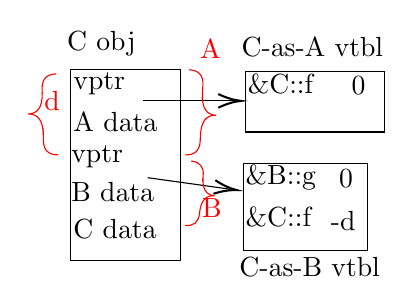
\begin{tikzpicture}[x=0.75pt,y=0.75pt,yscale=-1,xscale=1]
%uncomment if require: \path (0,719); %set diagram left start at 0, and has height of 719

%Shape: Rectangle [id:dp0013717648795982251] 
\draw   (35,421) -- (88,421) -- (88,513) -- (35,513) -- cycle ;
%Shape: Rectangle [id:dp687854832434939] 
\draw   (119,422) -- (186,422) -- (186,451) -- (119,451) -- cycle ;
%Shape: Rectangle [id:dp7436844684942457] 
\draw   (118,466) -- (178,466) -- (178,508) -- (118,508) -- cycle ;
%Straight Lines [id:da7863846979004839] 
\draw    (70,436) -- (115,436) ;
\draw [shift={(117,436)}, rotate = 180] [color={rgb, 255:red, 0; green, 0; blue, 0 }  ][line width=0.75]    (10.93,-3.29) .. controls (6.95,-1.4) and (3.31,-0.3) .. (0,0) .. controls (3.31,0.3) and (6.95,1.4) .. (10.93,3.29)   ;
%Straight Lines [id:da6152704816573378] 
\draw    (72,473) -- (113.02,478.72) ;
\draw [shift={(115,479)}, rotate = 187.94] [color={rgb, 255:red, 0; green, 0; blue, 0 }  ][line width=0.75]    (10.93,-3.29) .. controls (6.95,-1.4) and (3.31,-0.3) .. (0,0) .. controls (3.31,0.3) and (6.95,1.4) .. (10.93,3.29)   ;
%Shape: Brace [id:dp0646553096211897] 
\draw  [color={rgb, 255:red, 255; green, 0; blue, 0 }  ,draw opacity=1 ] (28,423) .. controls (23.33,423.12) and (21.06,425.51) .. (21.18,430.18) -- (21.23,432.14) .. controls (21.4,438.81) and (19.16,442.2) .. (14.49,442.32) .. controls (19.16,442.2) and (21.58,445.47) .. (21.75,452.14)(21.67,449.14) -- (21.82,455.18) .. controls (21.94,459.85) and (24.33,462.12) .. (29,462) ;
%Shape: Brace [id:dp7777929204704227] 
\draw  [color={rgb, 255:red, 255; green, 0; blue, 0 }  ,draw opacity=1 ] (90,462) .. controls (94.66,462.23) and (97.1,460.01) .. (97.33,455.35) -- (97.47,452.58) .. controls (97.79,445.93) and (100.28,442.71) .. (104.95,442.94) .. controls (100.28,442.71) and (98.11,439.27) .. (98.44,432.61)(98.29,435.61) -- (98.65,428.33) .. controls (98.88,423.67) and (96.66,421.23) .. (92,421) ;
%Shape: Brace [id:dp29878544281007513] 
\draw  [color={rgb, 255:red, 255; green, 0; blue, 0 }  ,draw opacity=1 ] (90,496) .. controls (94.25,496.41) and (96.59,494.49) .. (97,490.24) -- (97,490.24) .. controls (97.59,484.16) and (100.01,481.33) .. (104.27,481.74) .. controls (100.01,481.33) and (98.18,478.08) .. (98.77,472)(98.5,474.74) -- (98.77,472) .. controls (99.18,467.75) and (97.25,465.41) .. (93,465) ;

% Text Node
\draw (119,422) node [anchor=north west][inner sep=0.75pt]   [align=left] {\&C::f};
% Text Node
\draw (35,421) node [anchor=north west][inner sep=0.75pt]   [align=left] {vptr};
% Text Node
\draw (35,440) node [anchor=north west][inner sep=0.75pt]   [align=left] {A data};
% Text Node
\draw (34,456) node [anchor=north west][inner sep=0.75pt]   [align=left] {vptr};
% Text Node
\draw (34,474) node [anchor=north west][inner sep=0.75pt]   [align=left] {B data};
% Text Node
\draw (35,492) node [anchor=north west][inner sep=0.75pt]   [align=left] {C data};
% Text Node
\draw (32,401) node [anchor=north west][inner sep=0.75pt]   [align=left] {C obj};
% Text Node
\draw (116,404) node [anchor=north west][inner sep=0.75pt]   [align=left] {C-as-A vtbl};
% Text Node
\draw (115,510) node [anchor=north west][inner sep=0.75pt]   [align=left] {C-as-B vtbl};
% Text Node
\draw (169,423) node [anchor=north west][inner sep=0.75pt]   [align=left] {0};
% Text Node
\draw (118,466) node [anchor=north west][inner sep=0.75pt]   [align=left] {\&B::g};
% Text Node
\draw (118,486) node [anchor=north west][inner sep=0.75pt]   [align=left] {\&C::f};
% Text Node
\draw (163,468) node [anchor=north west][inner sep=0.75pt]   [align=left] {0};
% Text Node
\draw (159,488) node [anchor=north west][inner sep=0.75pt]   [align=left] {\mbox{-}d};
% Text Node
\draw (21,430) node [anchor=north west][inner sep=0.75pt]  [color={rgb, 255:red, 255; green, 0; blue, 0 }  ,opacity=1 ] [align=left] {d};
% Text Node
\draw (96,405) node [anchor=north west][inner sep=0.75pt]  [color={rgb, 255:red, 255; green, 0; blue, 0 }  ,opacity=1 ] [align=left] {A};
% Text Node
\draw (97,482) node [anchor=north west][inner sep=0.75pt]  [color={rgb, 255:red, 255; green, 0; blue, 0 }  ,opacity=1 ] [align=left] {B};


\end{tikzpicture}

    \tikzset{every picture/.style={line width=0.75pt}} %set default line width to 0.75pt        

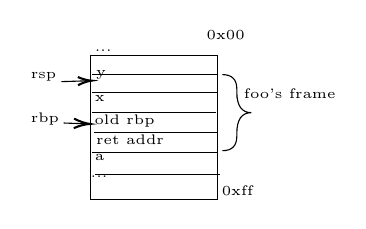
\begin{tikzpicture}[x=0.75pt,y=0.75pt,yscale=-1,xscale=1]
%uncomment if require: \path (0,719); %set diagram left start at 0, and has height of 719

%Shape: Rectangle [id:dp09641394842131779] 
\draw   (407,332.33) -- (468,332.33) -- (468,402) -- (407,402) -- cycle ;
%Straight Lines [id:da6006770345705227] 
\draw    (407.67,350.33) -- (427.67,350.33) -- (467.67,350.33) ;
%Straight Lines [id:da15594765253623044] 
\draw    (407.5,360) -- (467.5,360) ;
%Straight Lines [id:da21110838355177608] 
\draw    (408.33,369.67) -- (468.33,369.67) ;
%Straight Lines [id:da6903923726693459] 
\draw    (407.67,379) -- (467.67,379) ;
%Straight Lines [id:da620203852389054] 
\draw    (409,389.67) -- (469,389.67) ;
%Straight Lines [id:da43419176108852553] 
\draw    (407.67,341.67) -- (467.67,341.67) ;
%Shape: Brace [id:dp32753352461992913] 
\draw   (470.33,378.33) .. controls (475,378.33) and (477.33,376) .. (477.33,371.33) -- (477.33,370) .. controls (477.33,363.33) and (479.66,360) .. (484.33,360) .. controls (479.66,360) and (477.33,356.67) .. (477.33,350)(477.33,353) -- (477.33,348.67) .. controls (477.33,344) and (475,341.67) .. (470.33,341.67) ;

% Text Node
\draw (407.5,360) node [anchor=north west][inner sep=0.75pt]  [font=\tiny] [align=left] {old rbp};
% Text Node
\draw (407.67,350.33) node [anchor=north west][inner sep=0.75pt]  [font=\tiny] [align=left] {x};
% Text Node
\draw (407.67,379) node [anchor=north west][inner sep=0.75pt]  [font=\tiny] [align=left] {a};
% Text Node
\draw (376.83,358.67) node [anchor=north west][inner sep=0.75pt]  [font=\tiny] [align=left] {rbp};
% Text Node
\draw (408.33,338.33) node [anchor=north west][inner sep=0.75pt]  [font=\tiny] [align=left] {y};
% Text Node
\draw (376.83,339.33) node [anchor=north west][inner sep=0.75pt]  [font=\tiny] [align=left] {rsp};
% Text Node
\draw (479.5,347.33) node [anchor=north west][inner sep=0.75pt]  [font=\tiny] [align=left] {foo's frame};
% Text Node
\draw (468.83,394) node [anchor=north west][inner sep=0.75pt]  [font=\tiny] [align=left] {0xff};
% Text Node
\draw (461.5,319.33) node [anchor=north west][inner sep=0.75pt]  [font=\tiny] [align=left] {0x00};
% Text Node
\draw (405.67,389) node [anchor=north west][inner sep=0.75pt]  [font=\tiny] [align=left] {...};
% Text Node
\draw (407.67,328.33) node [anchor=north west][inner sep=0.75pt]  [font=\tiny] [align=left] {...};
% Text Node
\draw (408.33,369.67) node [anchor=north west][inner sep=0.75pt]  [font=\tiny] [align=left] {ret addr};
% Connection
\draw    (393.83,364.99) -- (404.5,365.37) ;
\draw [shift={(406.5,365.44)}, rotate = 182.05] [color={rgb, 255:red, 0; green, 0; blue, 0 }  ][line width=0.75]    (7.65,-2.3) .. controls (4.86,-0.97) and (2.31,-0.21) .. (0,0) .. controls (2.31,0.21) and (4.86,0.98) .. (7.65,2.3)   ;
% Connection
\draw    (392.83,345.06) -- (405.33,344.66) ;
\draw [shift={(407.33,344.59)}, rotate = 178.15] [color={rgb, 255:red, 0; green, 0; blue, 0 }  ][line width=0.75]    (6.56,-1.97) .. controls (4.17,-0.84) and (1.99,-0.18) .. (0,0) .. controls (1.99,0.18) and (4.17,0.84) .. (6.56,1.97)   ;

\end{tikzpicture}

  \end{multicols*}

\end{multicols*}
\end{document}

% ____ FOOTER ______________________________________________________
% Content and Template: 
% original by Danny Camenisch (dcamenisch@inf.ethz.ch), 2022
% based on different summaries from many helpful people
